\section{Planification Microsoft Project}

Microsoft Project est un outil puissant, que nous apprenons tout juste à appréhender. Il nous offre un grand nombre de possibilités ainsi qu'une aide qui s'avérera utile dans le pilotage de notre projet. Nous avons retenu les informations les plus importantes qu'il synthétise.

\subsection{Chronologie du projet}
Cette vue (cf.\textsc{figure~\ref{fig:timeline}}) est la plus synthétique que nous ayons réalisée, elle donne une vue d’ensemble du projet ne comprenant que les plus grandes étapes. 
\begin{figure}
	\centering
	\caption{Chronologie générale}
		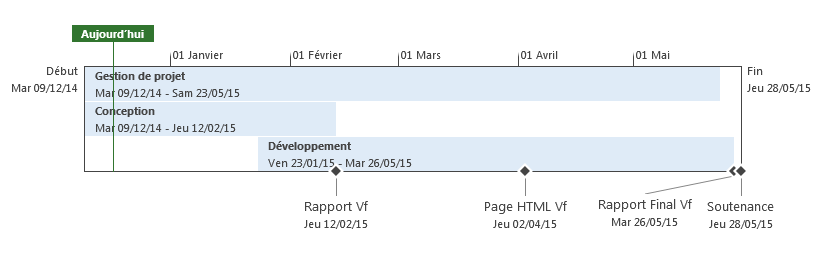
\includegraphics[width=\textwidth]{3-Planification/img/timeline.PNG}
	\label{fig:timeline}
\end{figure}


Une autre vue importante est le temps de travail cumulé (cf.\textsc{figure~\ref{fig:avancement}}) restant. Il est assez équilibré tout au long du projet avec toutefois quelques variations brusques autours des jalons précédemment définis.
\begin{figure}
	\centering
	\caption{Temps de travail cumulé restant}
		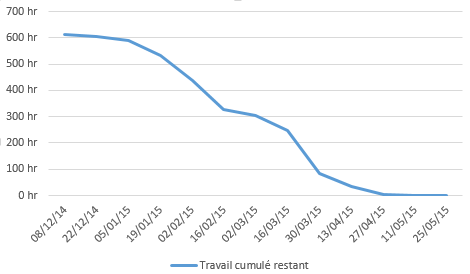
\includegraphics[width=\textwidth]{3-Planification/img/avancement.PNG}
	\label{fig:avancement}
\end{figure}


\subsection{Diagramme de Gantt}
Nous avons subdivisé notre projet en un ensemble de sous-tâches avec le plus de précision possible, en tentant de faire une estimation de la durée que chacune d'entre elle demanderait.

Le diagramme de Gantt (cf.\textsc{figure~\ref{fig:gantt}}) permet d'avoir une vue plus détaillée des différentes tâches du projet, ordonnancées en fonction de leur durée et de leur priorité. 
\begin{figure}
	\centering
	\caption{Diagramme de Gantt}
			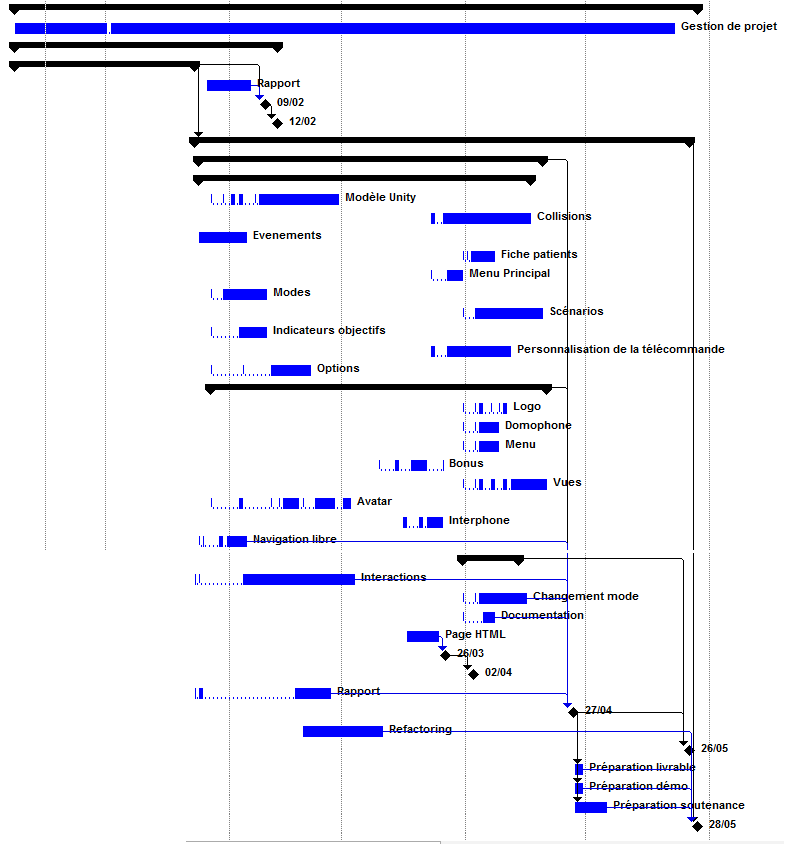
\includegraphics[width=\textwidth]{3-Planification/img/gantt.png}
	\label{fig:gantt}
\end{figure}
